% !TEX root = SystemTemplate.tex

\chapter{Overview and concept of operations}

The overview should take the form of an executive summary.  Give the reader a feel 
for the purpose of the document, what is contained in the document, and an idea 
of the purpose for the system or product. 


\section{Scope}
This document entails the design, implimentation and future plans for Crowd Control by BowTaps. 


\section{Purpose}
Crowd Control is a mobile application designed to ease the experence of going out though the implimentation of integrated group messaging, GPS tracking and group management features. Along with the features to manage your group at the event Crowd Control also gives suggestions of local events, restraunts and attraction. This allows the group to continue even when the next item on the agenda is a mystry. 


Even though Crowd Control is designed for the party sceen and people going out to events, it uses can be expanded to fit more purposes. Crowd Control can be used to help manage any kind of group at an event such as church groups or school field trips.


\subsection{Integrated Group Messaging}
Integrated group messaging is an important feature of Crowd Control. Integrated group messaging allows for communication between cross platform, different phone brands, and different carriers. This allows for seamless communicaton between users with out the issues associated with messaging such as messages not using the same format, messages not going to all recipiants, and messages with users in the group that you do no want to have your personal information.

\subsection{GPS Location services}
GPS allows for tracking of members in the group on a local map of the area. With this feature you will be able to keep track of anyone in the group off of their last GPS check in. This is useful to help locate members of the group that maybe lost or unable to be located. This feature will have the option of being able to opt out when the user does not want to have their location known to the group. When the users battary is low it will allow for the check in period to be extended or turned off to save battary life.

\subsection{Group Management Features}
The group management features allow for information to be shared with the group. A group management menu will allow for a group agenda to be posted as well as updates when the agenda changes. With the GPS features it will allow for the group leader to set way points for the group.  

\subsection{Suggestions}
Suggestions are both a plus for the user and our way of making a monitary developement. Suggestions are sponsored by local busnesses in the form of an ad. Altough these are not traditional ads, they are in the form of local points of intrest such as restraunts, bars, amusement parks, or bowling alllys. The possibilities are endless. With the suggestion method it will allow for our users to have helpful suggestions of places for their group to attend as well as exposure for the local busnesses that are sponsering Crowd Control.

\section{Systems Goals}
The goal of this application is to create a group management application with group messaging, GPS tracking, and group management freatures all under a data safe enviroment though encryption.

\section{System Overview and Diagram}
Provide a more detailed description of the major system components
without getting too detailed.  This section should contain a
high-level block and/or flow diagram of the system highlighting the
major components.  See Figure~\ref{systemdiagram}.  This is a floating
figure environment.  \LaTeX\ will try to put it close to where it was
typeset but will not allow the figure to be split if moving it can not
happen.  Figures, tables, algorithms and many other floating
environments are automatically numbered and placed in the appropriate
type of table of contents.  You can move these and the numbers will
update correctly.

\begin{figure}[tbh]
\begin{center}
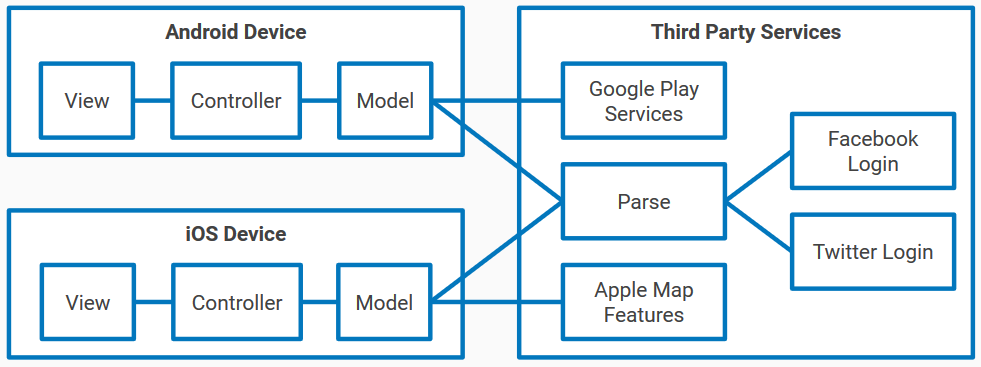
\includegraphics[width=0.75\textwidth]{designpictures/ModuleFlowDiagram.png}
\end{center}
\caption{Basic System Flow Diagram \label{ModuleFlowDiagram}}
\end{figure}

\section{Technologies Overview}
This section should contain a list of specific technologies used to
develop the system.  The list should contain the name of the
technology, brief description, link to reference material for further
understanding, and briefly how/where/why it was used in the system.
See Table~\ref{somenumbers}.  This is a floating table environment.
\LaTeX\ will try to put it close to where it was typeset but will not
allow the table to be split.

\begin{table}[tbh]
\caption{A sample Table ... some numbers. \label{somenumbers}}
\begin{center}
\begin{tabular}{|r|l|}
  \hline
  7C0 & hexadecimal \\
  3700 & octal \\ \cline{2-2}
  11111000000 & binary \\
  \hline \hline
  1984 & decimal \\
  \hline
\end{tabular}
\end{center}
\end{table}

